\section{GPU Implementation} \label{gpu-implementation}

\begin{figure}[htb]
  \centering
  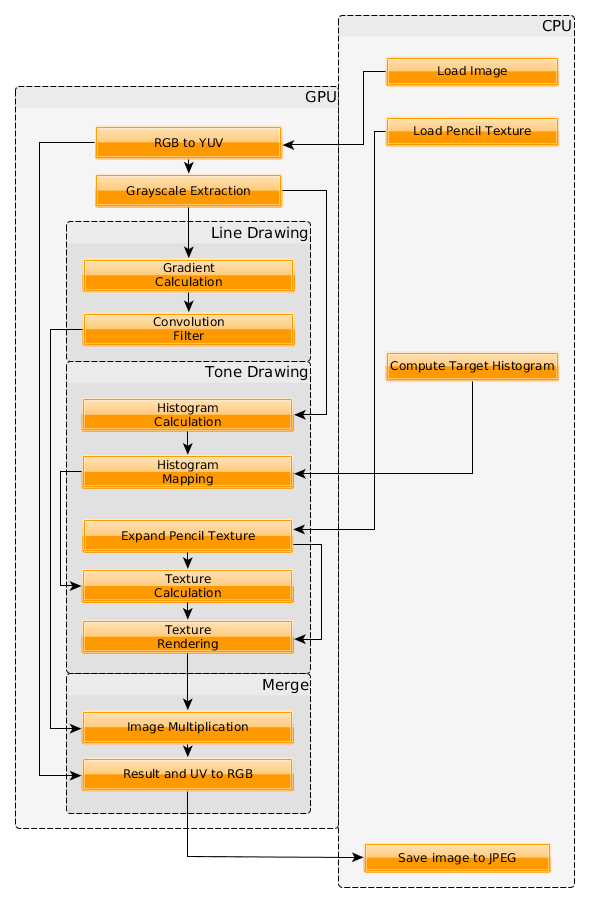
\includegraphics[width=0.5\textwidth]{images/pipeline.png}
  \caption{GPU and CPU pipeline of the implementation}
  \label{fig:pipeline}
\end{figure}

\autoref{fig:pipeline} displays the GPU and CPU pipeline of the implementation.
The first step loads the image, which happens on the CPU.  The conversion of
the image from RGB to YUV on the GPU is run in parallel with the loading of the
pencil textures on the CPU.  The next kernel extracts the grayscale version of
the image from the RGB to YUV result.  The grayscale version is used for the
gradient calculation, which is then fed into the convolution filter.  This
finalizes the line drawing step.  In preparation for the shading or tone drawing
step, the CPU is computing the target histogram using \autoref{eq:p}.  The histogram
calculation in the tone drawing step receives the grayscale version as the
input image. The result is then passed to the histogram mapping kernel,
together with the CPU-computed target histogram. Yet Another kernel expands the
hatching pattern image $H$ to image size. The expanded textures and the
tonal texture $J$ are used for the texture calculation. The last kernel
in the tone drawing section - the texture rendering kernel - computes the final
hatching texture for the image. The last two kernels merge line drawing and
hatching texture. One kernel combines the results of the line drawing and the
tone drawing step and generates the final image, the last kernel adds back the
colors if requested and converts the YUV back to RGB. The CPU takes care of
saving the image to disk again.

\subsection{Sketch Filter}
Calculating the grayscale image $I_g$ and gradient $G$ on the GPU is no big
challenge. However the efficient implementation of the line convolution
calculation is more interesting.

To calculate the value $L(x)$, first all $G_i(x)$ have to
be computed (see \autoref{eq:Gi}) and the maximum from all line convolution
results then has to be selected (see \autoref{eq:L}). The following paragraphs describe the
implementation of the Cuda-Kernel which computes $L$ directly from $G$ given
the desired line length, strength and count.

\paragraph{Compute the line convolutions} 
To compute the convolution result $G_i(x)$ for pixel $x$ and line $i$ all values of $G$
along the line segment $\mathscr{L}_i$ are collected and averaged. The
convolution-kernel of the line segment $\mathscr{L}_i$ can be described as 
\begin{align*}
  k_i(p) = \begin{cases}
    \frac{1}{\text{line length} \cdot \text{line strength}} & p \text{ is part
    of } \mathscr{L}_i\\
    0 & \text{otherwise}
  \end{cases}
\end{align*}
Collecting the right pixels for the right line is done by iterating over the
pixels of a horizontal line with the desired length and strength. This line
starts at $x$. Then the coordinates are rotated to get the pixels for line $i$.
The rotation angle depends on the line count, as the angle between two lines is
$\frac{360^{\circ}}{\text{line count}}$.  All line convolutions for one pixel
are calculated by a single thread. The results for a line is kept as maximum if
it is bigger than all its predecessors.

Finally in the inversion, a gamma correction and clipping is used to create the
final value for $L(x)$:
\begin{align*}
  L(x) = \max(255 - \max(G_i)^{\gamma}, 50)
\end{align*}
The $\gamma$ parameter can be used to intensify or weaken the lines.

\paragraph{Shared Memory}
The same pixel values from $G$ have to be loaded from neighboring quite often to
calculate all convolution results.  Therefore it makes sense to use shared memory
to speed up memory access.  Each pixel is calculated by a individual thread,
and as we can only use 1024 threads in one block we get blocks of size
$32\times32$, as shown in \autoref{fig:shared-memory}

\begin{figure}[htb]
  \centering
  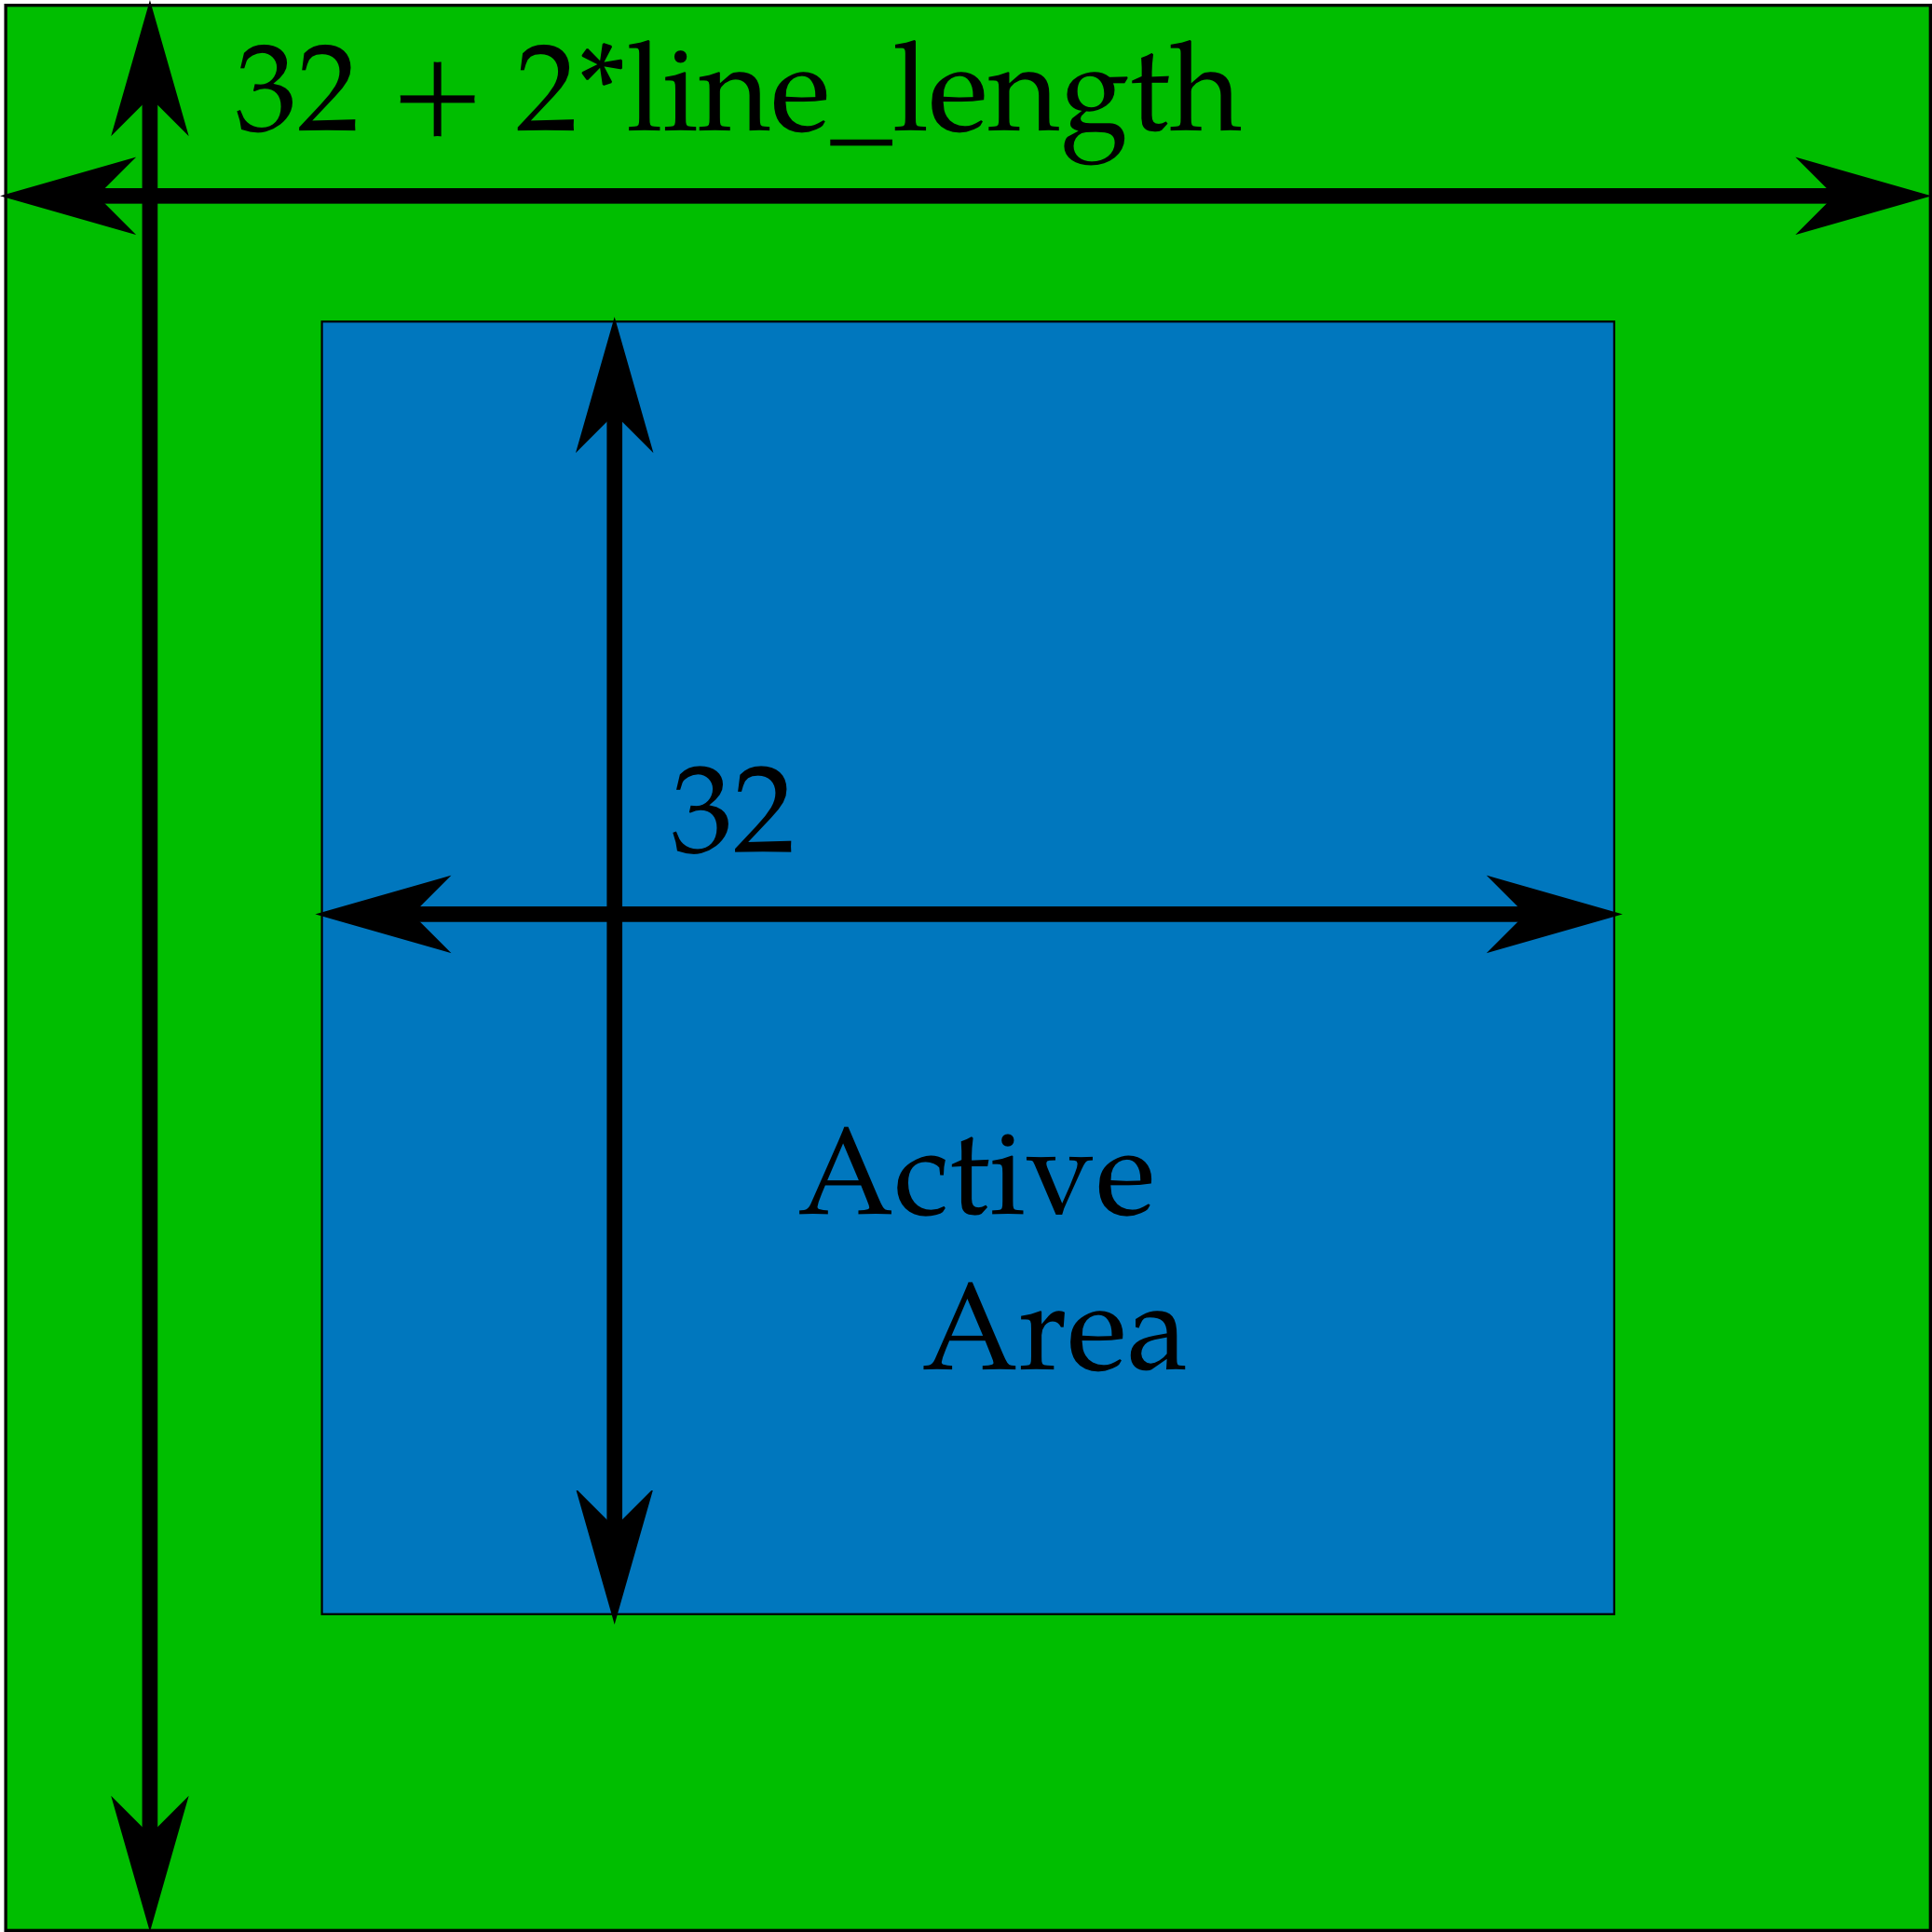
\includegraphics[width=0.2\textwidth]{images/shared-memory.png}
  \caption{Block dimension (blue) and shared memory dimension (green)}
  \label{fig:shared-memory}
\end{figure}

On our device the maximum size of shared memory per block is $48kb$, so we can
only store a $109\times109$ block of float values. Therefore only line
lengths up to 45 pixels are allowed which is more than enough for the purpose of
creating pencil sketches.

The data from $G$ is copied by assigning the thread number to the linear
indexes of the data. Because there is more data elements than threads, one
thread copies multiple data elements. The pattern is depicted in
\autoref{fig:shared-copy}.  \autoref{fig:shared-copy}.
\begin{figure}[htb]
  \centering
  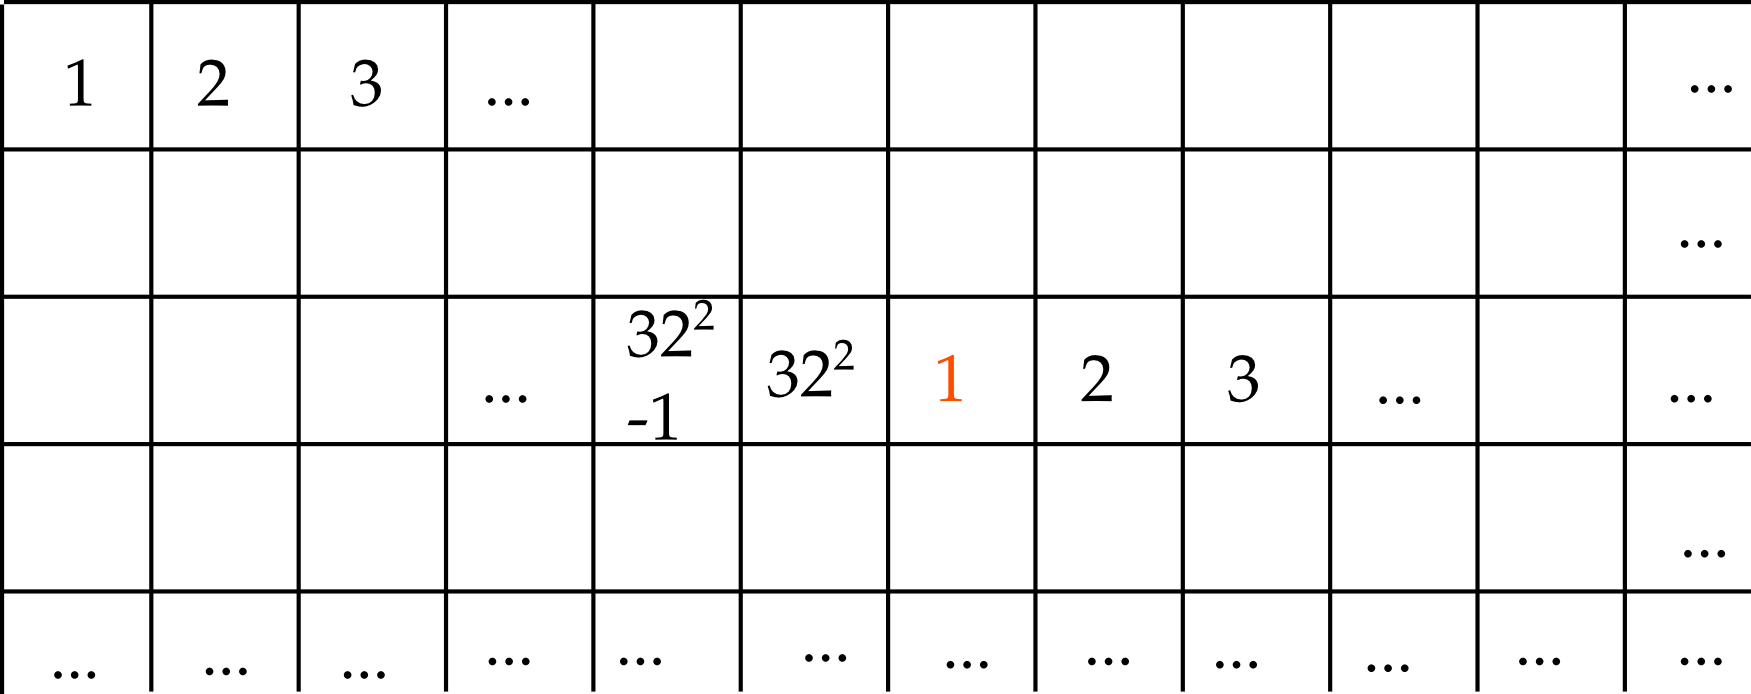
\includegraphics[width=0.5\textwidth]{images/shared-copy.png}
  \caption{Thread number assignment when copying the data from $G$ to shared memory.}
  \label{fig:shared-copy}
\end{figure}

The coordinate calculations for the line convolution computations are done such
that they generate the correct coordinates inside the shared memory block. Due to
the coordinate rotations the access patterns are very chaotic, which might lead
to unavoidable bank conflicts.



\subsection{Histogram}
The histogram calculation calculates a partial histogram within multiple blocks.
This is done in shared memory. Further more every block computes an additional
cumulative histogram using a parallel prefix sum. The partial results are being
combined at the end by 256 threads. They add the local results from shared
memory in to global memory using \texttt{atomicAdd}. As our histograms have
256 bins the needed shared memory size per block is only two times 256 Integers,
one for the simple histogram and one for the cumulative histogram.

\subsection{Histogram Matching}
Histogram matching is used to adjust the tone distribution of the 
image $I_g$ to match a specific target tone distribution. In this context, the
target tone distribution is artificially created using the model in
\autoref{eq:p}. This model creates a histogram which is similar to those of real
pencil sketches as explained above.

The cumulative target histogram is created on the CPU by simply applying
the parametric model to the values 0 to 255 and summing them up. This step is done
on the CPU as the target distribution only has to be evaluated 256 times which
is negligible effort and can be either be precomputed or done while the GPU is
busy with other steps of the pipeline.

Once this histogram is uploaded to the GPU it can be used together with
the histogram from the input image, which was created in the previous step, to
adjust the tones of the grayscale image. This is done in a kernel with one
thread per image pixel. A thread will then obtain the tone value of the pixel it
belongs to and look up it's cumulative probability value in the source histogram
map.  Afterwards, the cumulative target histogram is used inversely to find out
which tone the value corresponds to in it. The pixel is then set to the value
that was looked up. The lookup is done using binary search.
One would think that a binary search is inefficient when multiple threads
are executed in a warp and search for different values, but it really isn't.
Because the cumulative target histogram map only consist of 256 values,
the binary search will need at maximum $\log_2(256)=8$ loop runs to end
up at the correct value. As the threads are executed in a warp,
the branches might get executed in serial. However there is just one 
real branching operation inside the loop body which could double the
effort. Still, the total effort is negligible in contrast to a linear search
through the map with a worst case complexity of 256.

\subsection{Texturing}
The \autoref{eq:beta} has the same shape as a Tikhonov regularization and
therefore can be solved exactly the same way by solving the following normal
equation:
\begin{align}
  \underbrace{(A A^T + \lambda \cdot \Gamma \Gamma^T)}_{A^*} x = \underbrace{A^T
  b}_{b^*}
  \label{eq:tikhonov}
\end{align}
$x$, in our case, is the solution image $\beta$ in vector shape. $A$ is a diagonal matrix.
Each diagonal element corresponds to one pixel in $\ln(H)$. $b$ is the
vectorized $\ln(J)$ image and $\Gamma$ is a diagonal matrix with two diagonals
representing the gradient operator, if multiplied to a vectorized image.

The iterative Conjugate Gradient solver from the cuda sparse library
(\texttt{cusp}) is used to solve the linear system $A^* x = b^*$.

To do so the input images $\ln(J)$ and $\ln(H)$ are downloaded from the GPU,
fed into diagonal matrices from \texttt{cusp} and then uploaded again to solve the
equation. After that the result is downloaded and uploaded again in our regular
data representation for the final composition with the line image $L$.

Matrix $A*$ and vector $b^*$ (\autoref{eq:tikhonov}) could be calculated using
\texttt{cusp}. Therefore it's necessary to upload $\ln(H)$, $\ln(H)$ and $\Gamma$, and
use the matrix operations included in \texttt{cusp} to calculate the
matrix-matrix and matrix-vector multiplications. However it is much more
effective to construct $A^*$ and $b^*$ on the CPU and upload only those two
objects, because \texttt{cusp} needs an output target matrix for each operation.
So a lot of unnecessary memory would be needed to be allocated and used for the
calculations on the GPU. Due to the nice structure of the matrices, $A^*$ and
$b^*$  can be
calculated in $\mathcal{O}(n)$, with $n =$ number of pixel in the input image.
This is illustrated for $A^*$ in \autoref{fig:matrix-mult}. The closed form of
$b^*$ is:
\begin{align*}
  b^*(i) = \ln(J(i)) \cdot \ln(H(i))
\end{align*}

\begin{figure}[htb]
  \centering
  {\small
  \begin{align*}
    A*= \begin{pmatrix}
      a & 0 & -\lambda & 0 & 0 & 0 & 0 & \dots\\
      0 & b & 0 & -\lambda & 0 & 0 & 0 & \dots\\
      -\lambda & 0 & b & 0 & -\lambda & 0 & 0 & \dots\\
      0 & -\lambda & 0 & b & 0 & -\lambda & 0 & \dots\\
      0 & 0 & -\lambda & 0 & b & 0 & -\lambda & \ddots\\
      \vdots& &  &  &\ddots  \\
      0 & 0 & \dots & 0 & -\lambda & 0 & b & 0 & -\lambda\\
      0 & 0 & \dots & 0 & 0 &-\lambda & 0 & b & 0\\
      0 & 0 & \dots & 0 & 0 & 0 &-\lambda & 0 & a \\
    \end{pmatrix}
  \end{align*}
}
  \caption{Closed form for Matrix $A^*$. Substitute $a = \lambda +
  \ln(H(i))^2$ and substitute $b = 2\lambda + \ln(H(i))^2$ with $i$ being the line
in the matrix.}
  \label{fig:matrix-mult}
\end{figure}

According to our tests assembling the Matrix on the CPU makes the filter
approximately two times faster compared to the GPU method.
